\documentclass[10pt,pdf,aspectratio=169]{beamer}
\usepackage[T1,T2A]{fontenc}
% Входная кодировка utf-8
\usepackage[utf8]{inputenc}
% Поддержка русского и английского. В частности переносы
\usepackage[english,russian]{babel}

% Theme for beamer presentation.
\usepackage{beamerthemesplit}
% Other themes include: beamerthemebars, beamerthemelined,
%                       beamerthemetree, beamerthemetreebars

\logo{
\includegraphics[width=1cm,height=1cm,keepaspectratio]{Logo_BSU.jpg}}
\title[Исследование гидроэкологических данных в пакете R]{Исследование гидроэкологических данных с использованием среды программирования R}    % Enter your title between curly braces
\author[Павлов Александр]{Павлов Александр Сергеевич}                 % Enter your name between curly braces
\institute{Кафедра Теории Вероятностей и Математической Статистики}      % Enter your institute name between curly braces
\date{\today}                    % Enter the date or \today between curly braces

\begin{document}

% Creates title page of slide show using above information
\begin{frame}
  \titlepage
\end{frame}

% \section[План]{}

% % Creates table of contents slide incorporating
% % all \section and \subsection commands
% \begin{frame}
%   \tableofcontents
% \end{frame}


\section{}

\begin{frame}
  \frametitle{Постановка задачи}   % Insert frame title between curly braces

  \begin{itemize}
    \item Исследование и статистическая обработка гидроэкологических данных в пакете R
    \item Вычисление и анализ описательных статистик
    \item Проверка исходных данных на нормальность
    \item Идентификация законов распределения
    \item Корреляционный анализ
    \item Регрессионный анализ
    \item Вариограммный анализ
    \item Кригинг
  \end{itemize}
\end{frame}

\section{Первичный анализ}


\begin{frame}
  \frametitle{Исходные данные}   % Insert frame title between curly braces
  \begin{columns}[c]
  \column{2in}  % slides are 3in high by 5in wide
  Исходные данные получены от учебно-научного центра <<Нарочанская биологическая станция им. Г.Г.Винберга>> .

  На рисунке представлена выборка наблюдений за температурой воды в июле месяце в период с 1975 по 2012 годы.
  \column{3in}
  \framebox{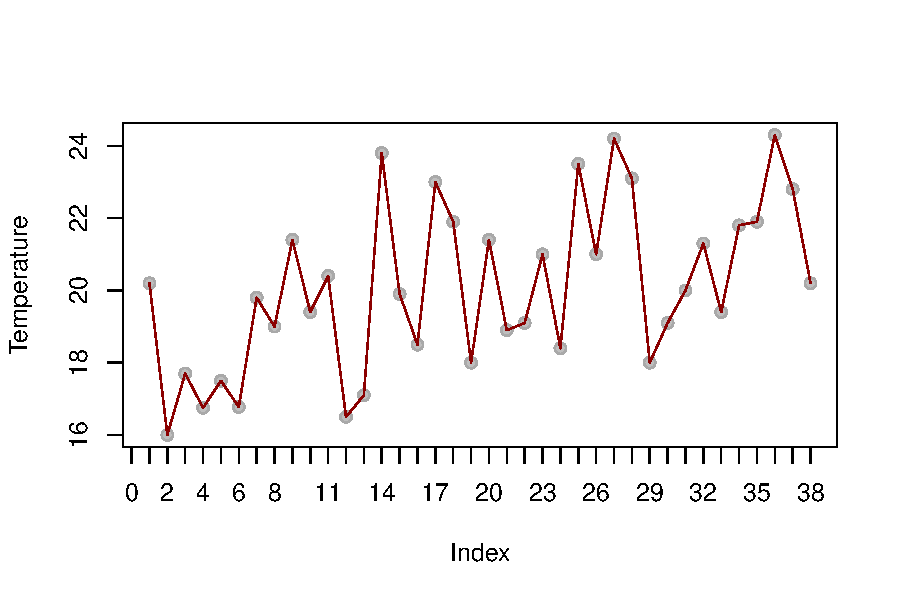
\includegraphics[width=3in]{../figures/temperature-ts-first-overview.pdf}
  }
  \end{columns}
\end{frame}

\subsection{Описательные статистики}

\begin{frame}
  \frametitle{Основные описательные статистики}   % Insert frame title between curly braces

  \input{../out/dstats_slides.tex}

\end{frame}

\subsection{Проверка на нормальность}

\begin{frame}
  \frametitle{Гистограмма наблюдаемых температур}   % Insert frame title between curly braces
   \begin{columns}[c]
   \column{4.5in}
  \includegraphics[width=4.5in]{../figures/article/hist.png}
  \end{columns}
\end{frame}

\begin{frame}
  \frametitle{График квантилей}   % Insert frame title between curly braces
   \begin{columns}[c]
   \column{4.5in}
  \includegraphics[width=4.5in]{../figures/article/qq.png}
  \end{columns}
\end{frame}

\begin{frame}
  \frametitle{Статистические критерии в R}   % Insert frame title between curly braces
   \begin{columns}[c]
   \column{2.2in}
   \textit{> shapiro.test()}:
   \begin{verbatim} 

	Shapiro-Wilk normality test

data:  Temperature
W = 0.9742, p-value = 0.5685

\end{verbatim}
   \column{2in}
  \textit{> pearson.test()}:
   \begin{verbatim} 

	Pearson chi-square normality test

data:  Temperature
P = 2.8, p-value = 0.8335

\end{verbatim}
  \end{columns}
\end{frame}


\section{Корреляционный анализ}

\subsection{Проверка наличия зависимости между температурой воды и временем}
\begin{frame}
  \frametitle{Диаграмма рассеяния}   % Insert frame title between curly braces
  \begin{columns}[c]
  \column{2in}  % slides are 3in high by 5in wide
  \begin{itemize}
  \item<1-> Выборочный коэффициент корреляции: $r_{xt}=0.52$
  \item<2-> При уровне значимости $\alpha=0.05$ выборочный коэффициент является значимым
  \end{itemize}
  \column{3in}
  \framebox{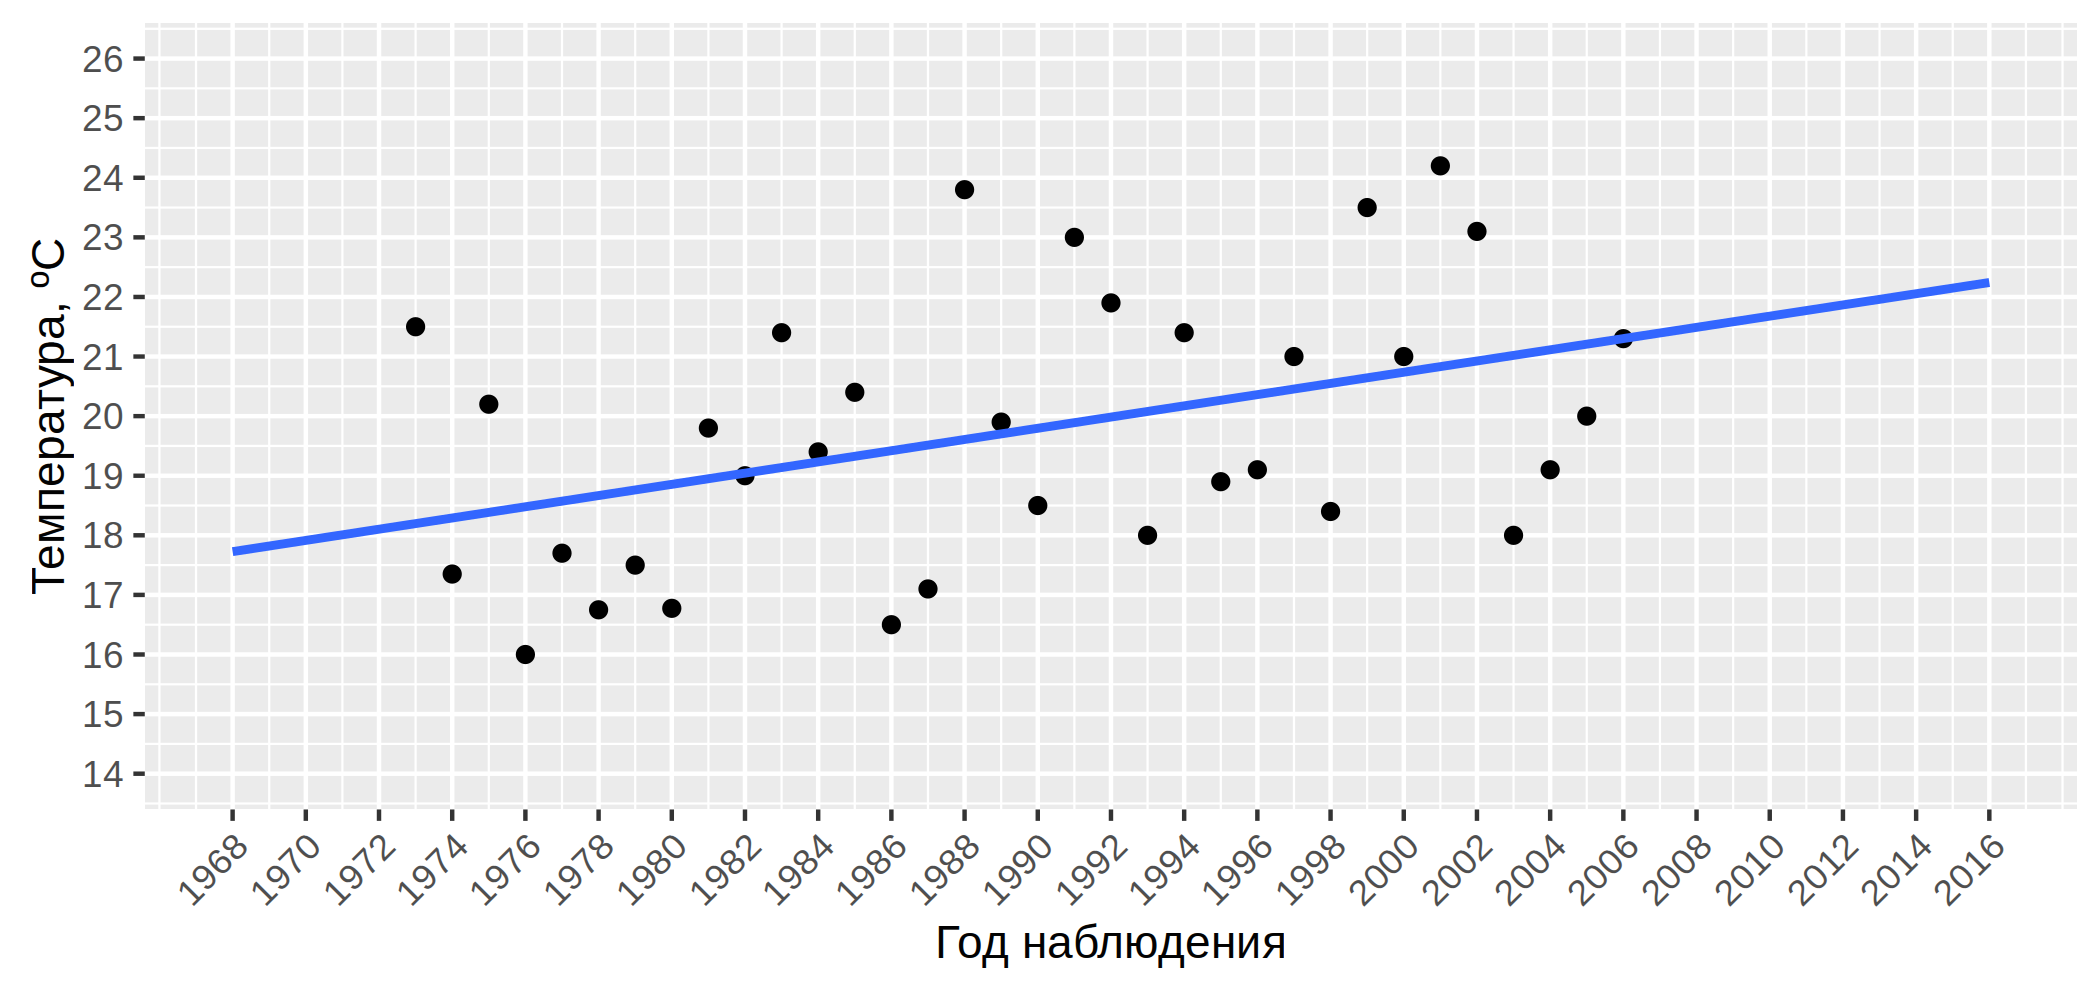
\includegraphics[width=3in]{../figures/article/scatterplot.png}}
  \end{columns}
\end{frame}

\subsection{Проверка значимости выборочного коэффициента корреляции}
\begin{frame}
  \frametitle{Проверка критерия значимости средствами пакета R}   % Insert frame title between curly braces
  \textit{> cor.test(method=``pearson'')}
   \begin{verbatim} 

	Pearson's product-moment correlation

data:  Temperature and Date
t = 3.6801, df = 36, p-value = 0.0007579
alternative hypothesis: true correlation is not equal to 0
95 percent confidence interval:
 0.2439316 0.7218701
sample estimates:
      cor 
0.5228432 

\end{verbatim}
\end{frame}

\section{Регрессионный анализ}

\subsection{Регрессионная модель}
\begin{frame}
  \frametitle{Временной ряд}   % Insert frame title between curly braces
  \begin{columns}[c]
  \column{2in}  % slides are 3in high by 5in wide
  \begin{itemize}
  \item<1-> Модель временного ряда: $X = T + E$
  \item<2-> Уравнение тренда: $x = 0.108t + 17.98$
  \end{itemize}
  \column{3in}
  \framebox{\includegraphics[width=3in]{../figures/article/ts.png}}
  \end{columns}
\end{frame}

\subsection{Качество регрессионной модели}
\begin{frame}
  \frametitle{Оценка модели}   % Insert frame title between curly braces
  \begin{itemize}
    \item<1-> С помощью критерия Стьюдента доказана значимость коэффициентов модели регрессии
    \item<2-> F-критерий Фишера при уровне значимости $\alpha = 0.05$ показал адекватность модели
    \item<3-> Точность модели невысока, посколько коэффициент детерминации $\eta^2_{x(t)} = 0.275$
  \end{itemize}
\end{frame}

\begin{frame}
  \frametitle{Прогноз}   % Insert frame title between curly braces
   \begin{columns}[c]
   \column{4.5in}
  \includegraphics[width=4.5in]{../figures/article/actvspred.png}
  \end{columns}
\end{frame}


\subsection{Анализ остатков}

\begin{frame}
  \frametitle{Автокорреляционная функция}   % Insert frame title between curly braces
   \begin{columns}[c]
   \column{4.5in}
  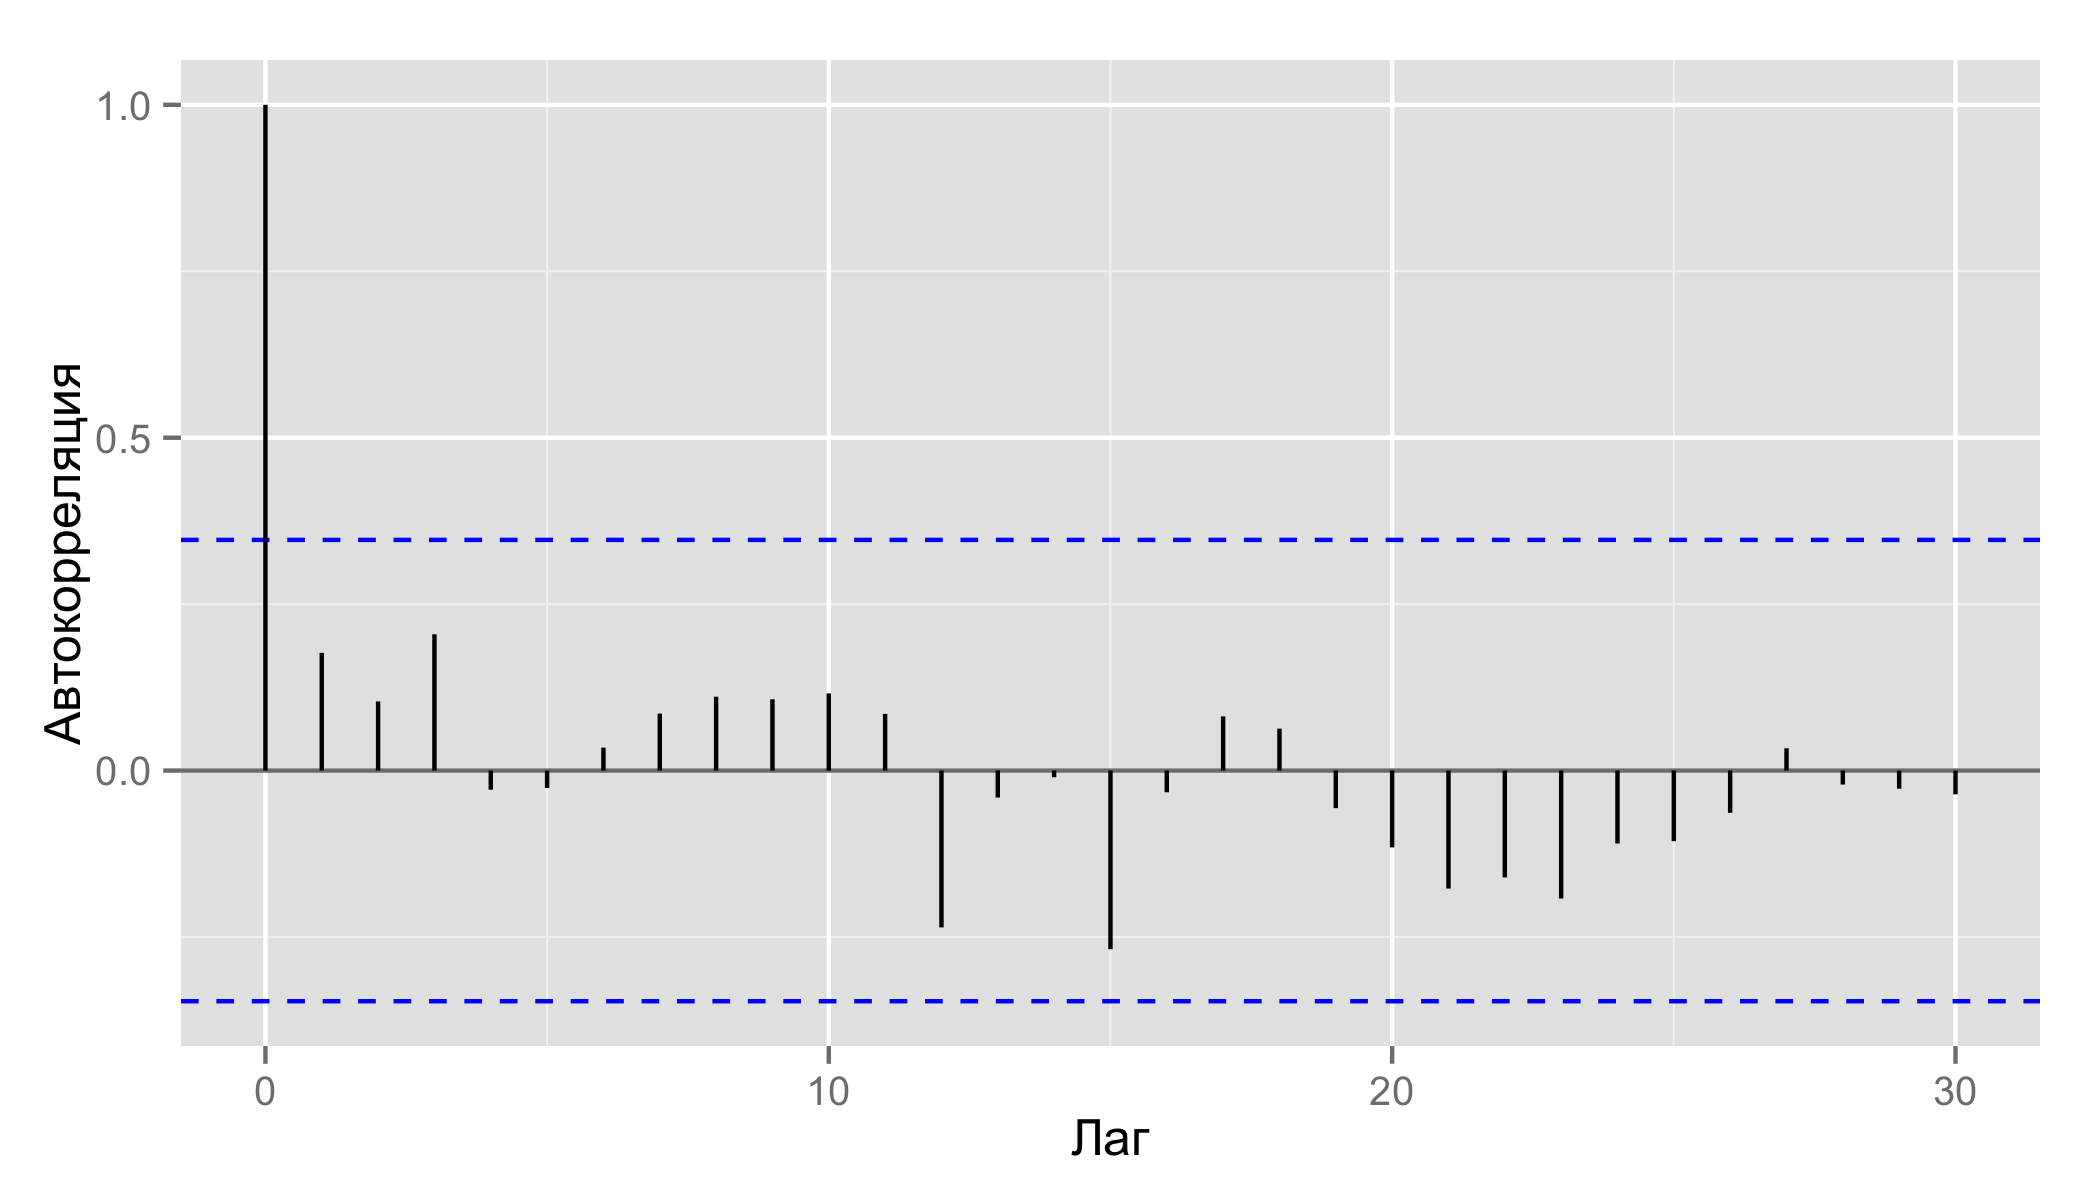
\includegraphics[width=4.5in]{../figures/article/acf.png}
  \end{columns}
\end{frame}

\section{Вариограммный анализ}

\subsection{Вариограмма}

\begin{frame}
  \frametitle{График экспериментальной вариограммы}   % Insert frame title between curly braces
   \begin{columns}[c]
   \column{4.5in}
  \includegraphics[width=4.5in]{../figures/article/variog1.png}
  \end{columns}
\end{frame}

\begin{frame}
  \frametitle{График экспериментальной вариограммы с подобранной моделью}   % Insert frame title between curly braces
  \begin{columns}[c]
  \column{2in}  % slides are 3in high by 5in wide
  Параметры модели:
  \begin{itemize}
  \item Модель: Сферическая с эффектом самородков
  \item Эффект самородков: $3.82$
  \item Порог: $4.22$
  \item Ранг: $4.19$
  \end{itemize}
  \column{3in}
  \framebox{\includegraphics[width=3in]{../figures/article/variog.png}}
  \end{columns}
\end{frame}

\subsection{Кригинг}
\begin{frame}
  \frametitle{Прогнозирование методом ординарного кригинга}   % Insert frame title between curly braces
   \begin{columns}[c]
   \column{4.5in}
  \includegraphics[width=4.5in]{../figures/article/actvspredpred.png}
  \end{columns}
\end{frame}

\subsection{}
\begin{frame}
  \frametitle{}   % Insert frame title between curly braces
   \begin{columns}[c]
   \column{1.3in}
  Спасибо за внимание
  \end{columns}
\end{frame}
\end{document}